\documentclass[twocolumn, 11pt]{article}%
\usepackage{amsmath, amssymb, esint, gensymb, hyperref, mathtools}
\usepackage{graphicx, cuted, geometry, float, scalerel, xcolor, xfrac}
\usepackage{enumitem}


\geometry{
    a4paper,
    total={170mm,260mm},
}

\begin{document}

\begin{strip}
  \vspace*{\dimexpr-\stripsep}
  \begin{center}
      \Large\textbf{FISIKA 2}\\
      \large{Pertemuan 1 - Minggu 11 (190055)}\\
      \large{\today}
   \end{center}
\end{strip}

\section{Gaya Gerak Listrik Induksi}
Lanjutannya minggu lalu.

\subsection{Induktansi Timbal Balik}%
Dua kumpran masing masing dialiri arus listrik I1  dan I2 seperti ditunjukkan pada Gambar
\begin{center}
    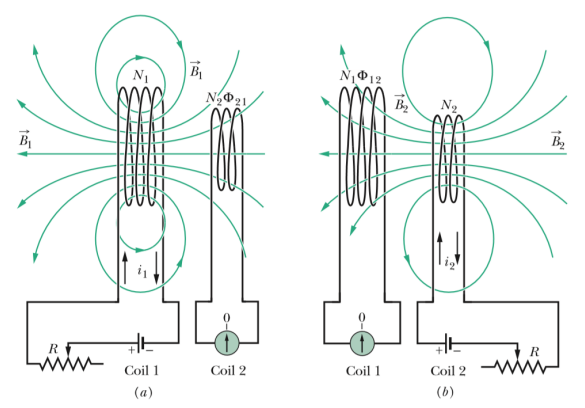
\includegraphics[width=200px]{1.png}
\end{center}

Pada gambar (a) ketika kumparan 1 dialiri arus maka $B_1$ akan menembus
kumparan 2, sebaliknya Ketika kuparan 2 (gambar b) dialiri arus maka
$B_2$ akan menembus kumparan 1, sehingga:

\[\Phi_{21} =B_1\ A_2\]
\[\Phi_{12} =B_2\ A_1\]\\

\textbf{PADA KUMPARAN 1}\\
$\Phi_{12}$ = fluks pada kawat 1 oleh kawat 2\\
$\Phi_{12} = k_2\ I_2$

\begin{align*}
    \epsilon_1 &=-N_1 \frac{d\Phi_{12}}{dt}\\
    \epsilon_1 &=-N_1 \frac{d(k_2\ I_2)}{dt}\\
    \epsilon_1 &=-N_1\ k_2 \frac{dI_2}{dt}\\
\end{align*}

dengan
\[M=N_1\ k_2\]

Jadi pada kumparan satu
\[\epsilon_1 = -M \frac{dI_2}{dt} \]

\textbf{PADA KUMPARAN 2}\\
$\Phi_{21}$ = fluks pada kawat 2 oleh kawat 1\\
$\Phi_{21} = k_1\ I_1$

\begin{align*}
    \epsilon_2 &=-N_2 \frac{d\Phi_{21}}{dt}\\
    \epsilon_2 &=-N_2 \frac{d(k_1\ I_1)}{dt}\\
    \epsilon_2 &=-N_2\ k_1 \frac{dI_1}{dt}\\
\end{align*}

dengan
\[M=N_2\ k_1\]

Jadi pada kumparan kedua
\[\epsilon_2 = -M \frac{dI_1}{dt} \]

Induktansi timbal balik disebut (M), atau sering juga disebut induktansi
silang, atau induktansi pasangan antara 2 kumparan. Nilai M pada kedua
kumparan tersebut sama, karena saling mempengaruhi

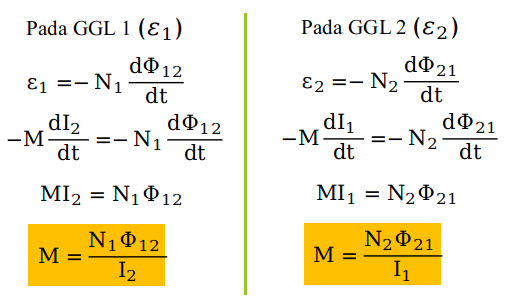
\includegraphics[width=200px]{2.png}

\subsection{Induktansi Diri}%
Selanjutnya Induktansi diri yang akan lebih banyak dibahas, dan
selanjutnya cukup akan disebut \textbf{Induktansi}.

$N_1=N_2=N$\\
$I_1=I_2=I$\\
$\Phi_{12}=\Phi_{21}=\Phi$\\
$\displaystyle M=L=N\frac{\Phi}{I}$\\

L juga disebut induktansi dengan satuan yang sama, yaitu \textbf{Henry
(H)}. Maka didapatkan Hukum Lenz dimana
\[\epsilon=-L\frac{dI}{dt}\]

\subsubsection{Energi Yang Tersimpan}%
\begin{center}
    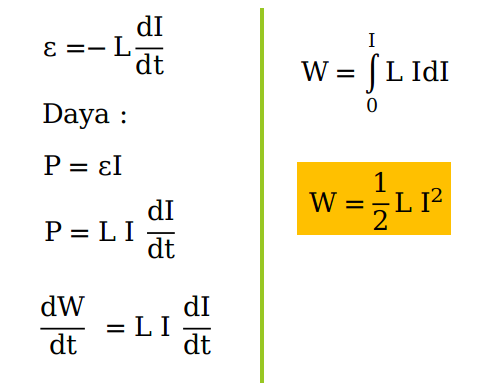
\includegraphics[width=170px]{3.png}
\end{center}

\subsubsection{Rapat Energi Induktor}%
Rapat energi adalah rumusan universal, bukan hanya berlaku di kumparan
selenoida, tapi juga berlaku di toroida, dll.
\begin{center}
    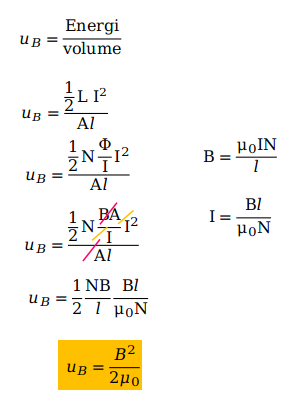
\includegraphics[width=180px]{4.png}
\end{center}

\subsection{Soal}%
\begin{center}
    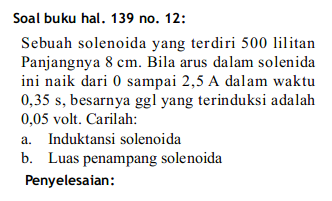
\includegraphics[width=200px]{5.png}
\end{center}

\begin{center}
    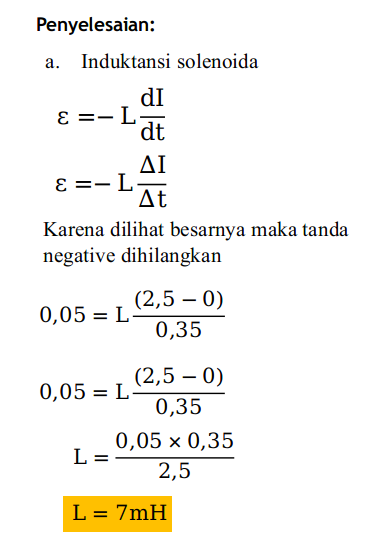
\includegraphics[width=160px]{6.png}
\end{center}

\begin{center}
    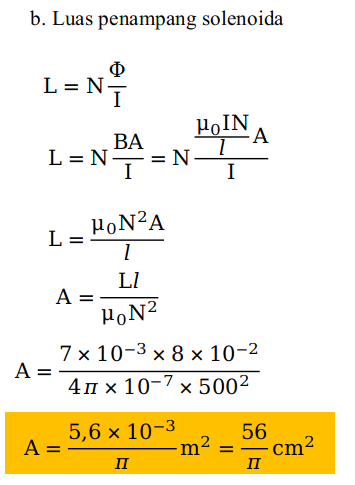
\includegraphics[width=160px]{7.png}
\end{center}

\begin{center}
    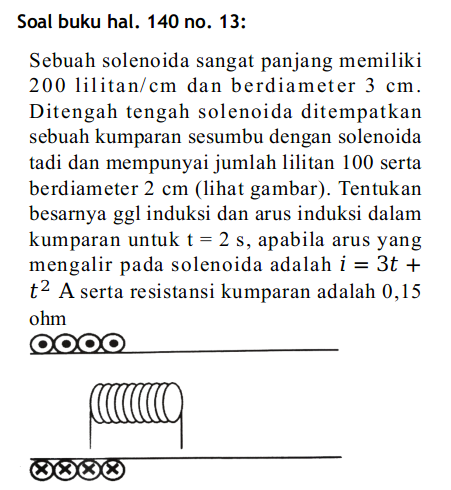
\includegraphics[width=180px]{8.png}
\end{center}

\begin{center}
    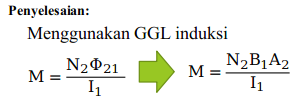
\includegraphics[width=140px]{9.png}
\end{center}

\begin{center}
    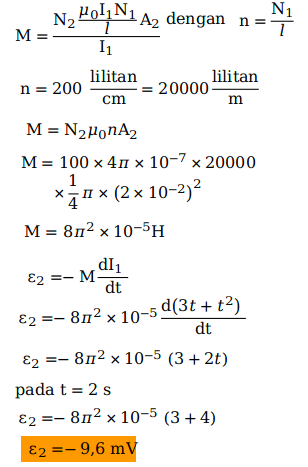
\includegraphics[width=170px]{10.png}
\end{center}

\begin{center}
    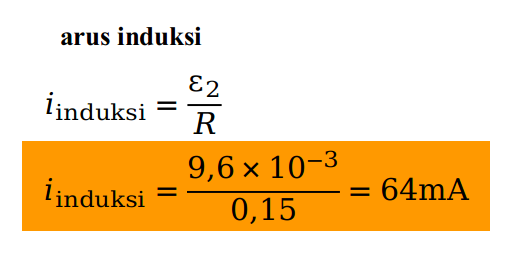
\includegraphics[width=170px]{11.png}
\end{center}

\begin{center}
    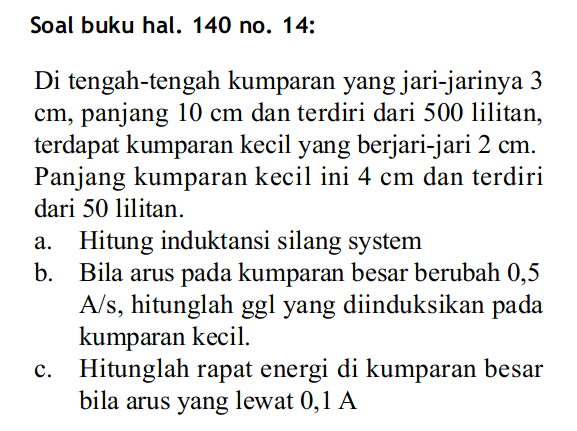
\includegraphics[width=200px]{12.png}
\end{center}

\begin{center}
    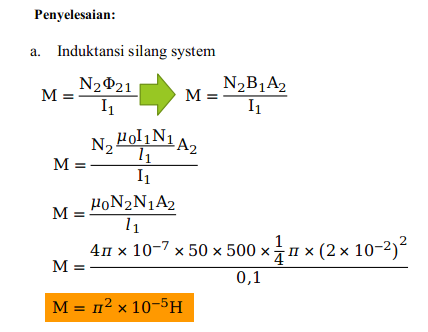
\includegraphics[width=210px]{13.png}
\end{center}

\begin{center}
    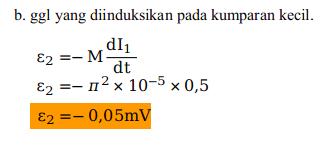
\includegraphics[width=180px]{14.png}
\end{center}

\begin{center}
    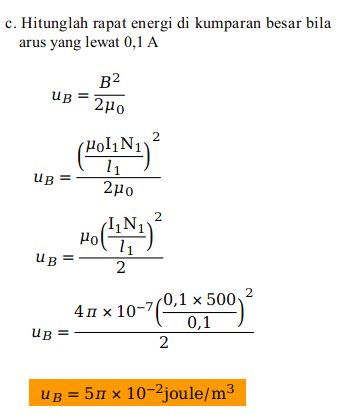
\includegraphics[width=200px]{15.png}
\end{center}

\subsection{Induktansi Silang antara Kawat Lurus dan Kawat Lurus}%
Perhitungan yang lengkap ada di Buku Diktat..

\begin{center}
    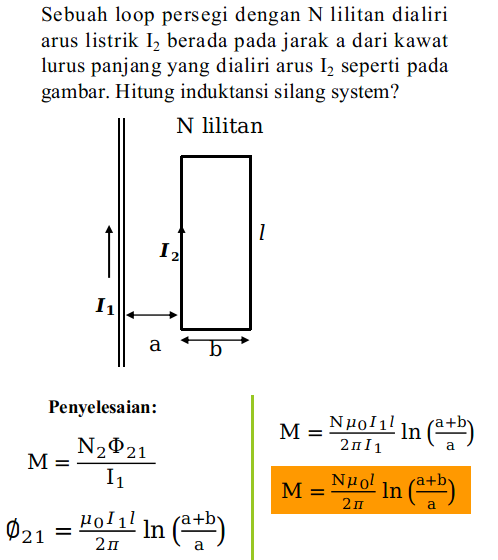
\includegraphics[width=200px]{16.png}
\end{center}

\end{document}
